\documentclass[aspectratio=169]{beamer}
\usepackage[utf8]{inputenc}
\usepackage{hyperref}
\usepackage{amsmath,amsfonts,amsthm,bm}
\usepackage{color}
\usepackage{graphicx} % Allows including images
\usepackage{subcaption}
\usepackage{booktabs} % Allows the use of \toprule, \midrule and \bottomrule in tables
\usepackage{tikz}
\usetikzlibrary{automata,positioning,shapes.geometric,shapes.misc,arrows}
%\usepackage{pgfplots}
\usepackage{listings}
\usepackage{courier}
\usepackage[version=4]{mhchem}
\usepackage{array}

\lstset{ %
    basicstyle=\scriptsize\ttfamily, % fonts that are used for the code
    breakatwhitespace=false,         % sets if automatic breaks should only happen at whitespace
%breaklines=true,                 % sets automatic line breaking
%captionpos=b,                    % sets the caption-position to bottom
    commentstyle=\color{gray}\textit,    % comment style
    keepspaces=true,                 % keeps spaces in text, useful for keeping indentation of code (possibly needs columns=flexible)
    keywordstyle=\color{blue},       % keyword style
    language=Python,                 % the language of the code
%otherkeywords={*,...},          % if you want to add more keywords to the set
    rulecolor=\color{black},         % if not set, the frame-color may be changed on line-breaks within not-black text (e.g. comments (green here))
    showspaces=false,                % show spaces everywhere adding particular underscores; it overrides 'showstringspaces'
    showstringspaces=false,          % underline spaces within strings only
    showtabs=false,                  % show tabs within strings adding particular underscores
    stringstyle=\color{red}, % string literal style
    tabsize=4,                       % sets default tabsize to 2 spaces
    columns=fixed                    % Using fixed column width (for e.g. nice alignment)
}

\hypersetup{
    colorlinks=true,
    linkcolor=red,
    filecolor=magenta,
    urlcolor=red,
}

\DeclareMathOperator*{\argmax}{argmax}
\DeclareMathOperator*{\argmin}{argmin}
\let \vec \mathbf

\newcommand{\classname}{NANO266}
\newcommand{\classyear}{Fall 2024}
\mode<presentation> {
    \usetheme{CambridgeUS}
    \setbeamertemplate{footline}[text line]{%
        \parbox{\linewidth}{\vspace*{-8pt}\classname\hfill\classyear\hfill\insertpagenumber}}

    %\setbeamertemplate{footline}[page number]
    \setbeamertemplate{navigation symbols}{}
}


\title[\classname AIMD]{\classname~- Ab initio Molecular Dynamics}

\author{Shyue Ping Ong}
\institute[UCSD]{University of California, San Diego\\
\medskip
}
\date{\classyear} % Date, can be changed to a custom date

\begin{document}


    \begin{frame}
        \titlepage % Print the title page as the first slide
    \end{frame}


    \begin{frame}{What is molecular dynamics (MD)?}
        Moving atomic nuclei by solving Newton’s equation of motion.

        \begin{equation*}
            M_I \ddot{\vec{R_I}} = - \frac{\partial E}{\partial \vec{R_I}} = \vec{F_I}[\{\vec{R_J}\}]
        \end{equation*}

        For $N$ nuclei, we have $3N$ positions and $3N$ velocities, i.e. a phase space of $6N$.

    \end{frame}


    \begin{frame}{Descriptions of the potential energy surface}

        \begin{columns}
            \column{0.5\textwidth}
            \begin{figure}
                \centering
                \includegraphics[width=0.6\linewidth]{lectures/figures/13_PES.png}
                \caption{Potential energy surface $E(\vec{R})$ and $F(\vec{R}) = E'(\vec{R})$.}
            \end{figure}
            \column{0.5\textwidth}
            Empirical force-fields
            \begin{itemize}
                \item Lennard-Jones potential
                \begin{itemize}

                    \item OK for rare gases
                    \item No chemistry
                    \item Only pair-wise and no directionality.
                \end{itemize}
                \item Embedded atom method (EAM)
                \begin{itemize}
                    \item Particularly effective for metals.
                    \item Can include many-body terms to incorporate dispersion, polarization, etc.
                \end{itemize}
            \end{itemize}

            Quantum mechanics!
            Expensive…, and surprisingly, not always the most accurate!

        \end{columns}

    \end{frame}

    \begin{frame}{2013 Nobel Prize in Chemistry}
        \begin{figure}
            \centering
            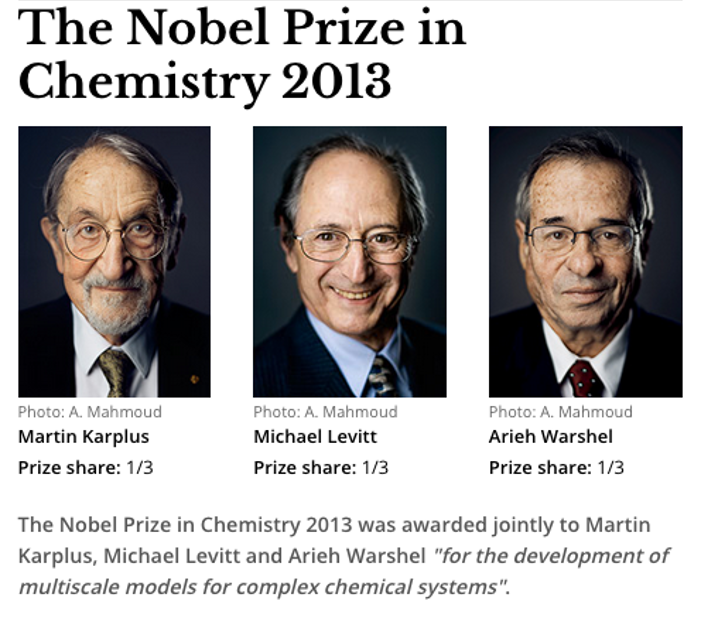
\includegraphics[width=0.4\linewidth]{lectures/figures/13-Nobel.png}
        \end{figure}
    \end{frame}

    \begin{frame}{Computational Experiment}
        \begin{figure}
            \centering
            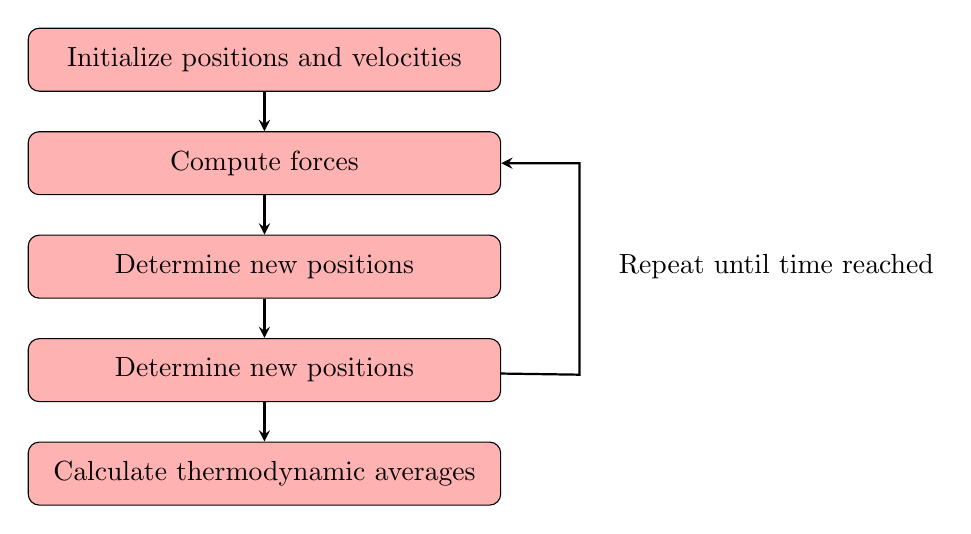
\begin{tikzpicture}[node distance=0.5cm]
                \tikzstyle{roundrect} = [rectangle, rounded corners, minimum width=6cm, minimum height=0.8cm,text centered, draw=black, fill=red!30]
                \tikzstyle{arrow} = [thick,->,>=stealth]
                \node (node1) [roundrect] {Initialize positions and velocities
                };
                \node (node2) [roundrect, below=of node1] {Compute forces
                };
                \node (node3) [roundrect, below=of node2] {Determine new positions
                };
                \node (node4) [roundrect, below=of node3] {Determine new positions
                };
                \node (node5) [roundrect, below=of node4] {Calculate thermodynamic averages};
                \node (annot) [right of=node3, node distance=6.5cm] {Repeat until time reached};

                \draw [arrow] (node1) -- (node2);
                \draw [arrow] (node2) -- (node3);
                \draw [arrow] (node3) -- (node4);
                \draw [arrow] (node4) -- (node5);
                \draw [arrow] (node4) -- (4, -4) |- (node2);

            \end{tikzpicture}
        \end{figure}
    \end{frame}


    \begin{frame}{Initialization}

        \begin{columns}
            \column{0.5\textwidth}
            \begin{equation*}
                M_I \ddot{\vec{R_I}} = - \frac{\partial E}{\partial \vec{R_I}} = \vec{F_I}[\{\vec{R_J}\}]
            \end{equation*}
            \begin{itemize}
                \item 2nd order PDF $\implies$ Needs initial positions and velocities.
                \item Positions: Reasonable guess based on structure, e.g., no overlap / short atomic distances.
                \item Velocities: Small initial velocity and steadily increase temperature (velocity scaling).
            \end{itemize}
            \column{0.5\textwidth}

            \begin{figure}
                \centering
                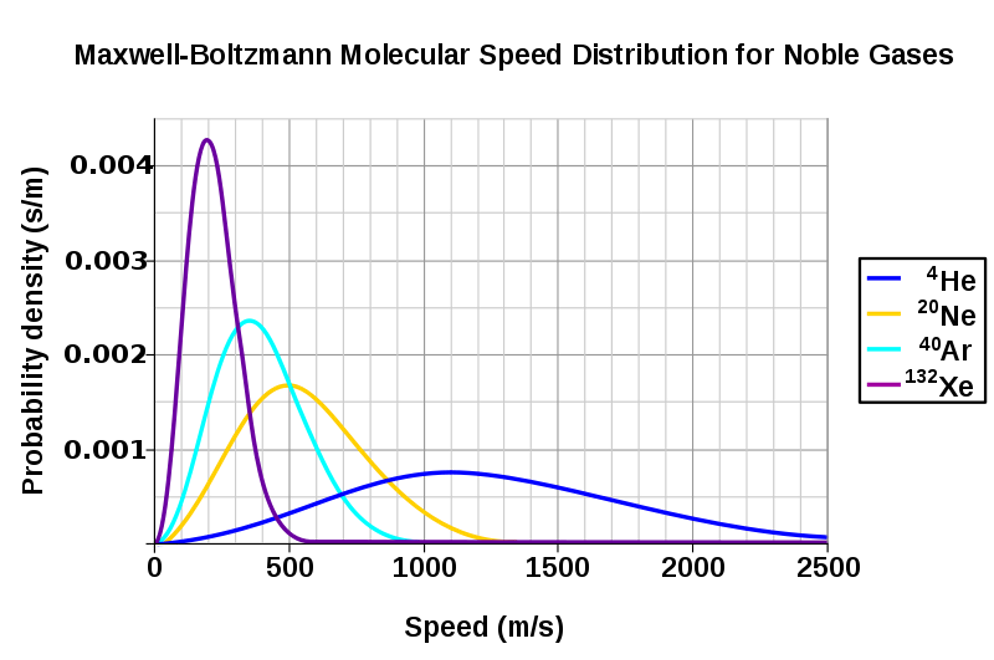
\includegraphics[width=0.8\linewidth]{lectures/figures/13-Maxwell_Boltzmann.png}
            \end{figure}
            \begin{equation*}
                f(\nu)=\sqrt{\left( \frac{m}{2\pi k_BT} \right)^3} 4\pi \nu^2 e^{-\frac{m\nu^2}{2k_BT}}
            \end{equation*}
        \end{columns}
    \end{frame}

    \begin{frame}{Ensembles}
        Microcanonical – Constant $N$, $V$, $E$\newline
        \newline
        Canonical – Constant $N$, $V$, $T$
        \begin{itemize}
            \item Temperature control achieved via thermostats
            \item Examples: velocity rescaling, Andersen thermostat, Nose-Hoover thermostat, Langevin dynamics, etc.
        \end{itemize}

        Grand canonical - Constant $\mu$, $V$, $T$

    \end{frame}

    \begin{frame}{Integrating the Equations of Motion - Verlet algorithm}
        \begin{eqnarray*}
            M_I \ddot{\vec{R_I}} & = &  \vec{F_I}[\{\vec{R_J}\}]\\
            \ddot{\vec{R_I}} & = & \frac{1}{M_I} \vec{F_I}[\{\vec{R_J}\}]\\
            \frac{[\vec{R_I}(t+\Delta t)-\vec{R_I}(t)]-[\vec{R_I}(t)-\vec{R_I}(t-\Delta t)]}{\Delta t} & = & \frac{1}{M_I} \vec{F_I}[\{\vec{R_J}\}]\\
            \vec{R_I}(t+\Delta t) & = & 2\vec{R_I}(t) + \vec{R_I}(t-\Delta t)]+\frac{\Delta t^2}{M_I} \vec{F_I}[\{\vec{R_J}\}]
        \end{eqnarray*}

        Key properties of Verlet algorithm
        \begin{itemize}
            \item Errors do not accumulate
            \item Energy is conserved
            \item Simulations are stable
        \end{itemize}
    \end{frame}

    \begin{frame}{Flavors of MD}
        Born-Oppenheimer (BOMD)
        \begin{itemize}
            \item Electrons stay in instantaneous ground state as nuclei move.
            \item Perform electronic SCF at each time step.
            \item Compute forces (Hellman-Feynman theorem).
            \item Move nuclei.
        \end{itemize}

        Car-Parrinello (CPMD)\cite{carUnifiedApproachMolecular1985}
        \begin{itemize}
            \item Treat ions and electrons as one unified system.
            \item Accomplished with fictitious kinetic energy for electrons.
            \item Avoids costly separate SCF for electrons at each step, but time step requried is much smaller than BO.
        \end{itemize}

    \end{frame}

    \begin{frame}{Anatomy of an MD Simulation}
        \begin{figure}
            \centering
            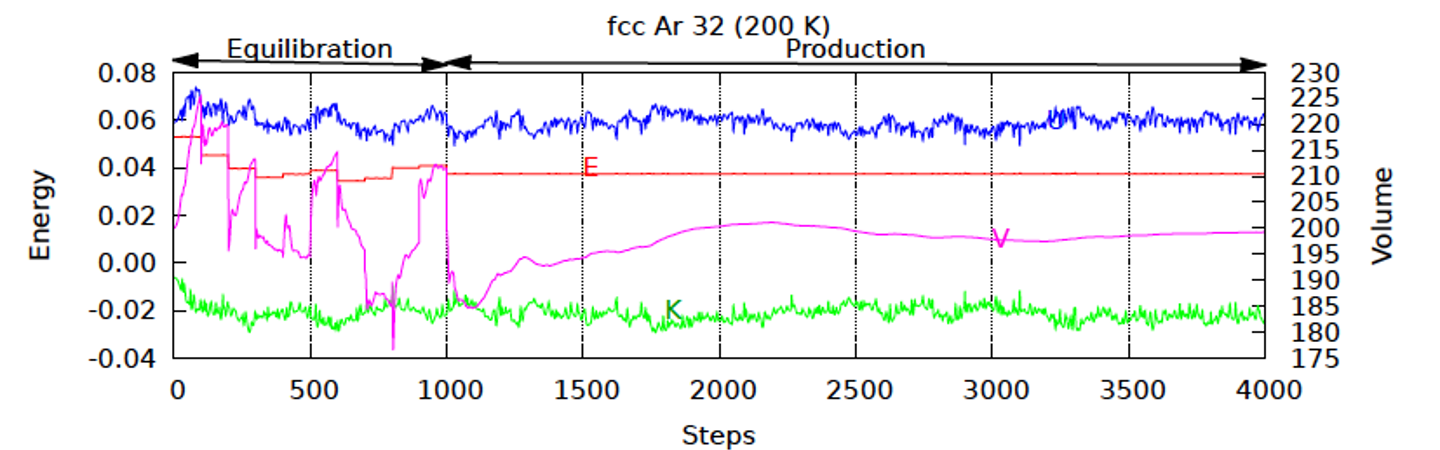
\includegraphics[width=\linewidth]{lectures/figures/13-MD_simulation.png}
            \caption{Typical energy and cell volume profile for an MD simulation.}
        \end{figure}
    \end{frame}

    \begin{frame}{Applications of MD simulations}
        \begin{columns}
            \column{0.7\textwidth}
            Thermodynamics from ensemble averages

            Real-time evolution
            \begin{itemize}
                \item Reactions
                \item Interaction of molecules on surfaces
                \item Trajectories of ions
            \end{itemize}

            Ground-state structures
            \begin{itemize}
                \item Geometry optimization is in fact a form of MD.
                \item For complex structures (e.g., low symmetry systems, interfaces, liquids, amorphous solids, etc.), MD can be used to determine low-energy structures
            \end{itemize}
            \column{0.3\textwidth}
            \begin{figure}
                \centering
                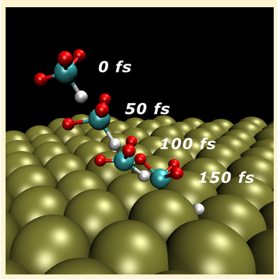
\includegraphics[width=\linewidth]{lectures/figures/13_CHD_Pt.png}
                \caption{AIMD of CHD 3 + Pt(111).\cite{nattinoInitioMolecularDynamics2014}}

            \end{figure}
        \end{columns}

    \end{frame}

    \begin{frame}{Thermodynamic Averages}
        Under ergodic hypothesis

        \begin{equation*}
            \left< A \right> = \sum_{\{\sigma\}} A_{\{\sigma\}} \frac{e^{-\frac{E[\{\sigma\}]}{k_BT}}}{Z} = \lim_{T\rightarrow \infty} \frac{1}{T} \int_0^T A(t) dt
        \end{equation*}

        Examples of averages
        \begin{itemize}
            \item Energy (potential, kinetic, total)
            \item Temperature
            \item Pressure
            \item Mean square displacements (diffusion)
            \item Radial distribution function
        \end{itemize}
    \end{frame}

    \begin{frame}{Correlation Functions from MD}
        Pair distribution function
        \begin{equation*}
            g(\vec{r}) = \frac{V}{N^2} \left< \sum_i \sum_{j \neq i} \delta(\vec{r} - \vec{r_{ij}}) \right>
        \end{equation*}

        Time correlation function

        \begin{columns}
            \column{0.5\textwidth}
            \begin{eqnarray*}
                \gamma & =  & \int_0^{\infty} \left< \dot{A}(t) \dot{A}(0) dt \right>
            \end{eqnarray*}
            Einstein relation (valid at large $t$)
            \begin{eqnarray*}
                2t \gamma & =  & \left< (A(t) - A(0))^2 \right> \mathrm{)}
            \end{eqnarray*}

            \column{0.5\textwidth}
            Example: Diffusion coefficient
            \begin{eqnarray*}
                D & =  & \int_0^{\infty} \left< \vec{v}(t) \vec{0}(0) dt \right> \\
                & =  & \frac{1}{2dt} \left< (\vec{r}(t) - \vec{r}(0))^2 \right>
            \end{eqnarray*}

        \end{columns}

    \end{frame}

    \begin{frame}{Example: Structure of Amorphous InP}
        \begin{figure}
            \centering
            \begin{subfigure}{0.3\textwidth}
                \centering
                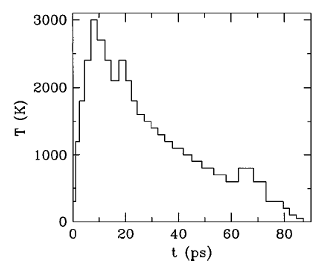
\includegraphics[width=\linewidth]{lectures/figures/13-InP_1.png}
                \caption{Thermal cycle of melt-quench process}
            \end{subfigure}
            \begin{subfigure}{0.3\textwidth}
                \centering
                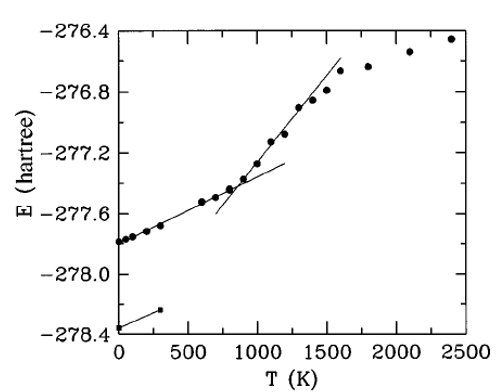
\includegraphics[width=\linewidth]{lectures/figures/13-InP_2.png}
                \caption{Total energy through liquid-glass transition.}
            \end{subfigure}
            \begin{subfigure}{0.3\textwidth}
                \centering
                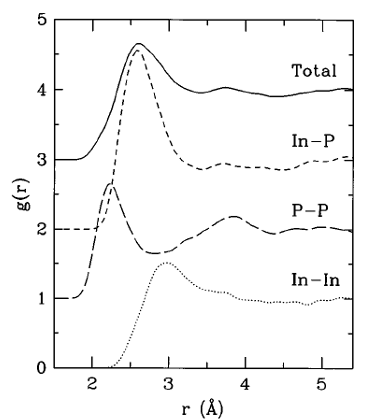
\includegraphics[width=\linewidth]{lectures/figures/13-InP_3.png}
                \caption{Partial and total RDF of liquid InP at 2100K.}
            \end{subfigure}
            \caption{\cite{lewisStructureElectronicProperties1998}}
            \label{fig}
        \end{figure}
    \end{frame}

    \begin{frame}{Example: Phase transition of LiOH}
        \begin{figure}
            \centering
            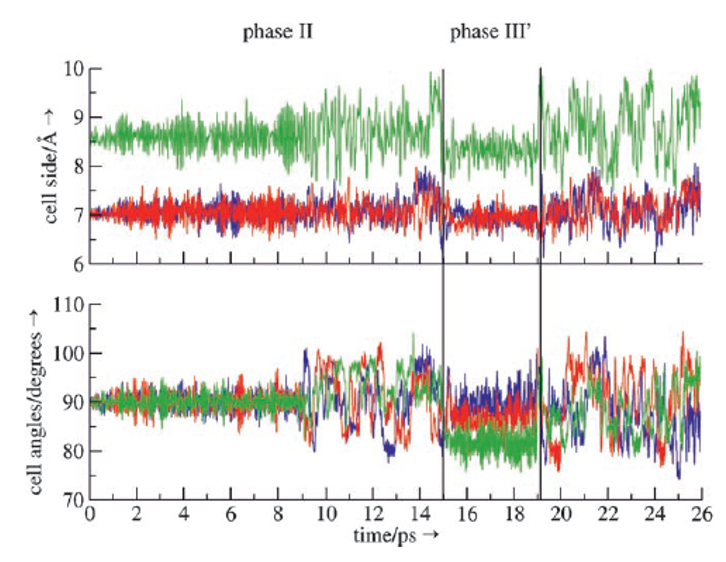
\includegraphics[width=0.5\linewidth]{lectures/figures/13-LiOH.png}
            \caption{Evolution of simulation cell parameters during MD.\cite{pagliaiLithiumHydroxidePhase2006}}
        \end{figure}
    \end{frame}

    \begin{frame}{Example: Water}
        \begin{figure}
            \centering
            \begin{subfigure}{0.45\textwidth}
                \centering
                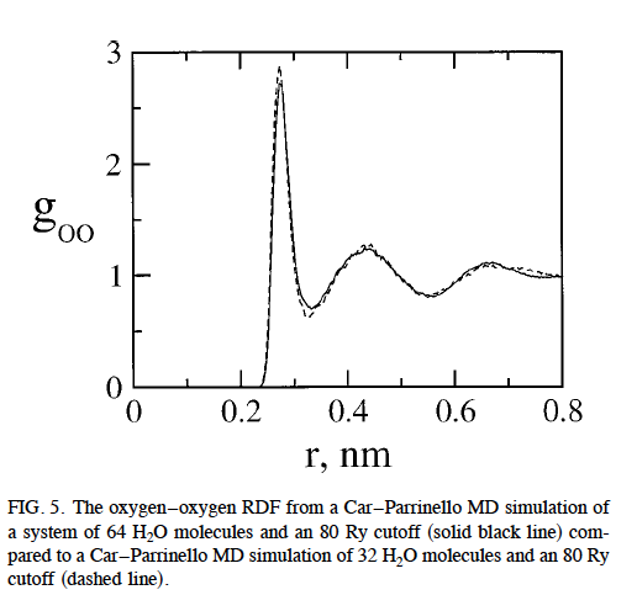
\includegraphics[width=\linewidth]{lectures/figures/13-H2O_1.png}
            \end{subfigure}
            \begin{subfigure}{0.2\textwidth}
                \centering
                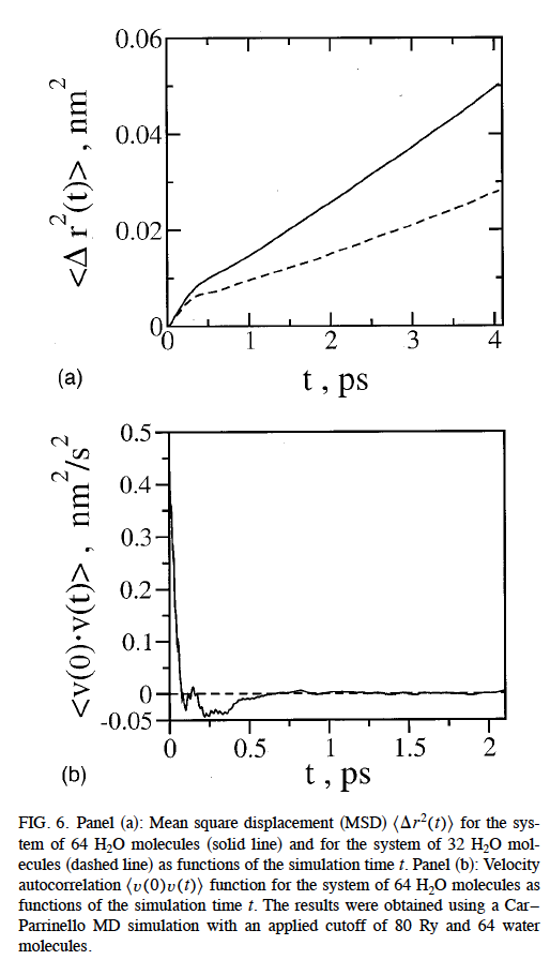
\includegraphics[width=\linewidth]{lectures/figures/13-H2O_2.png}
            \end{subfigure}
            \caption{CPMD simulations of water.\cite{izvekovCarParrinelloMolecularDynamics2002}}
            \label{fig}
        \end{figure}
    \end{frame}


    \begin{frame}{Example: Lithium superionic conductors}
        \begin{figure}
            \centering
            \begin{subfigure}{0.45\textwidth}
                \centering
                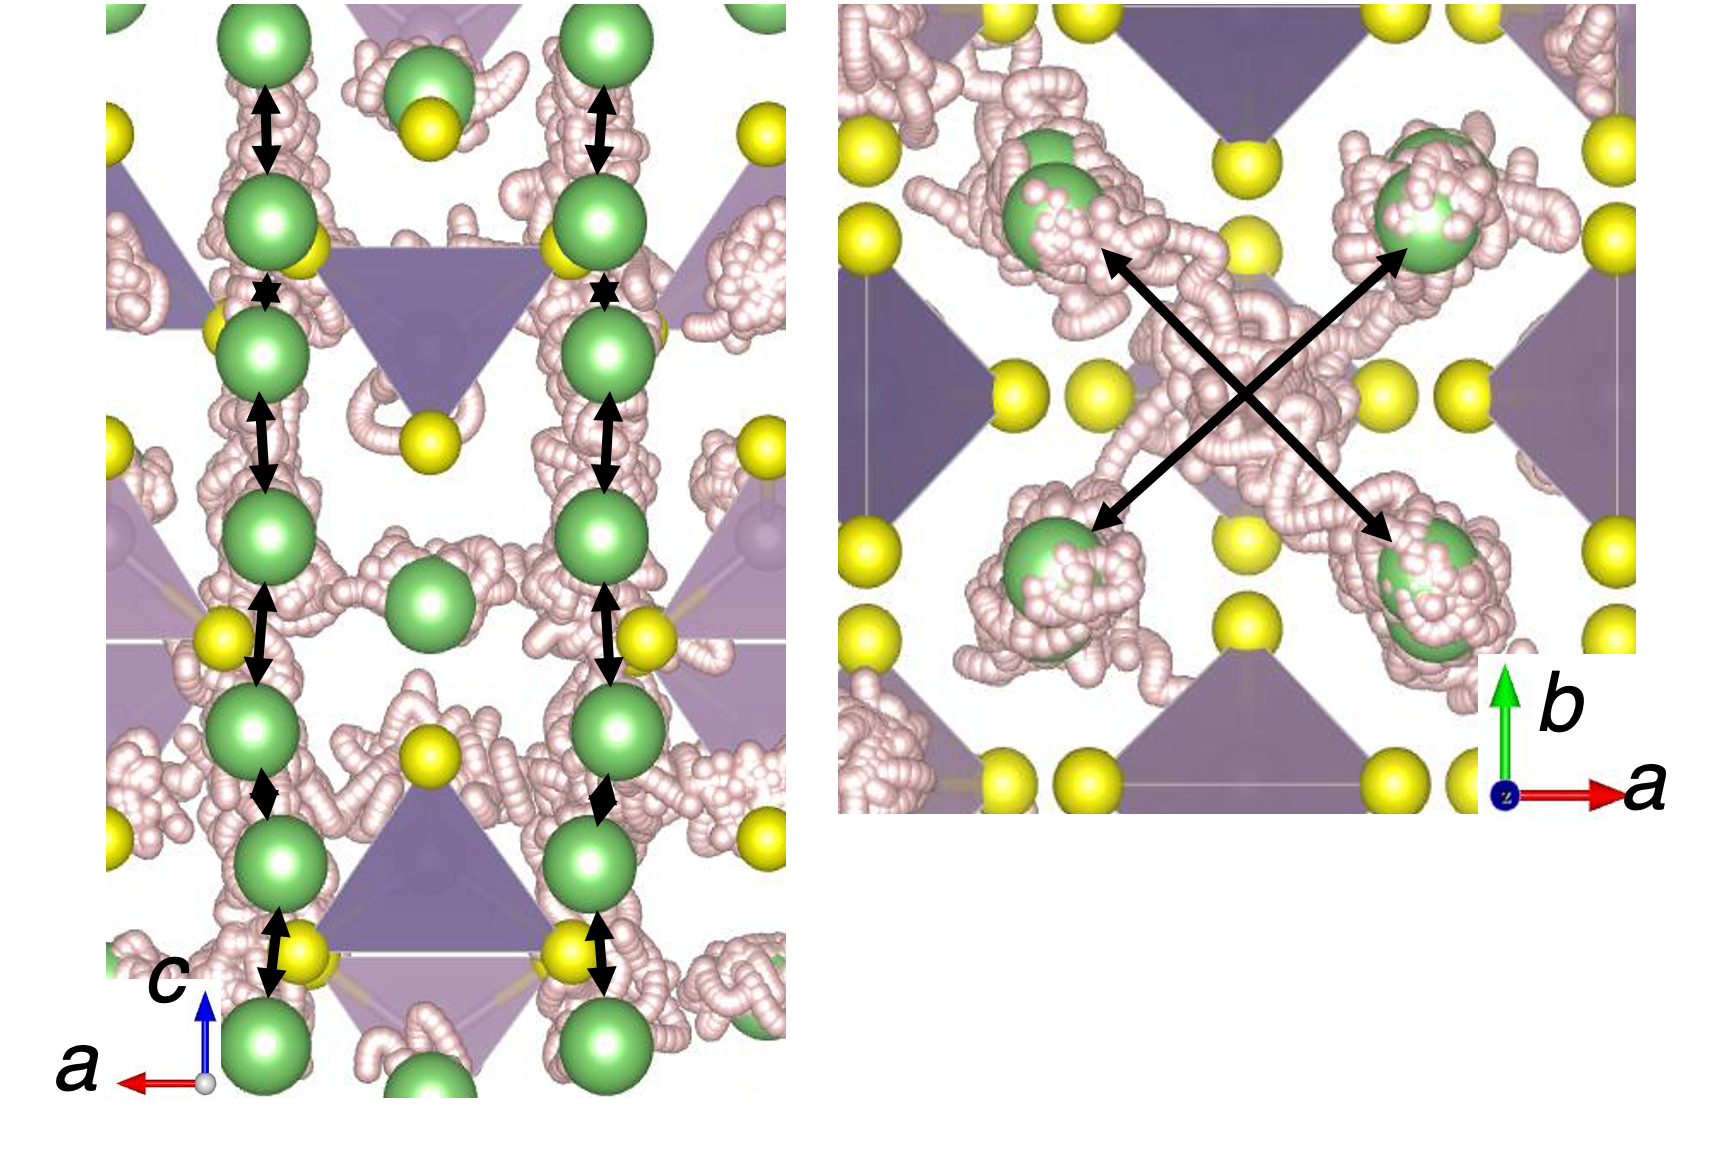
\includegraphics[width=0.9\linewidth]{lectures/figures/13-LGPS_1.png}
                \caption{Trace of Li motion at 900K, showing 3D diffusion. 1D conductors would be highly sensitive to blocking defects!}
            \end{subfigure}
            \begin{subfigure}{0.45\textwidth}
                \centering
                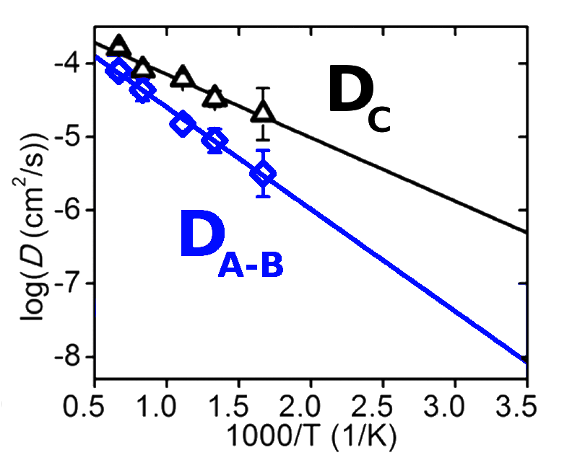
\includegraphics[width=0.8\linewidth]{lectures/figures/13-LGPS_2.png}
                \caption{Arrhenius Plot. Predicted: $E_a = 210$ meV. $\sigma = 13$ mS/cm. Experiment\cite{kamayaLithiumSuperionicConductor2011}: $E_a = 240$ meV, $\sigma = 12$ mS/cm.
                }
            \end{subfigure}
            \caption{AIMD study of \ce{Li10GeP2S12}.\cite{moFirstPrinciplesStudy2012}}
        \end{figure}
    \end{frame}

    \begin{frame}{Improving \ce{Li10GeP2S12}}
        \begin{figure}
            \centering    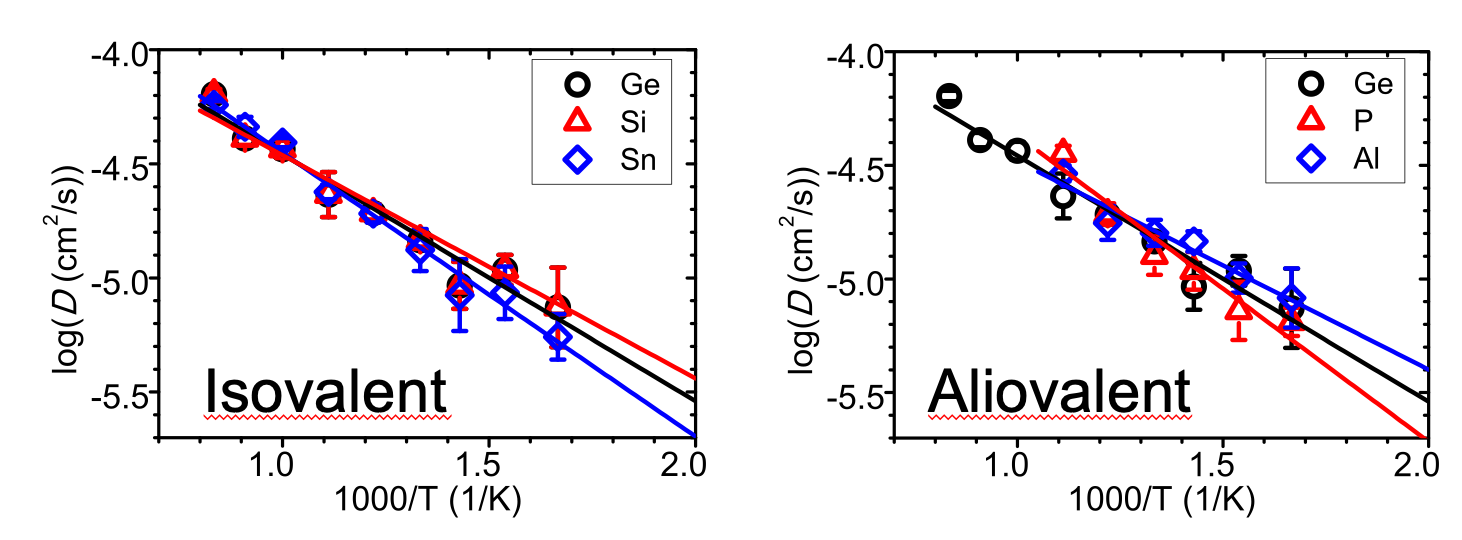
\includegraphics[width=0.65\linewidth]{lectures/figures/13-LMPS.png}
            \caption{Arrhenius plots for \ce{Li$_{10\pm1}$MP2X12} family of superionic conductors.\cite{ongPhaseStabilityElectrochemical2013}}
        \end{figure}

        \begin{table}[]
            \centering
            \begin{tabular}{c|c|c|c|c|c}
                & Ge  & Si  & Sn  & P   & Al  \\
                \hline
                $\sigma_{300K}$ (mS/cm) & 13  & 23  & 6   & 4   & 33  \\
                $E_a$ (meV)             & 210 & 200 & 240 & 260 & 180
            \end{tabular}
        \end{table}

    \end{frame}

    \begin{frame}{Example: Phonons from MD}
        \begin{columns}
            \column{0.5\textwidth}
            \begin{figure}
                \centering
                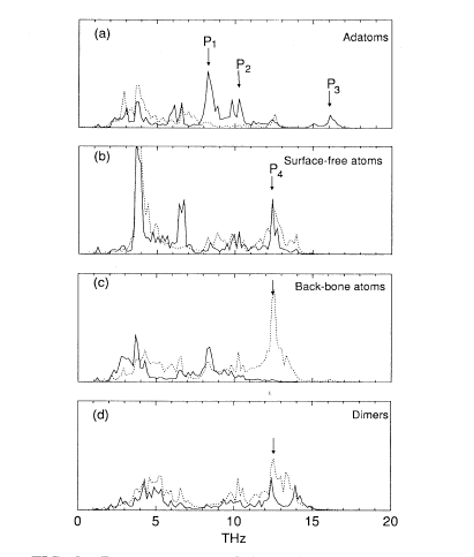
\includegraphics[width=0.7\linewidth]{lectures/figures/13-Phonons_MD.png}
            \end{figure}
            \column{0.5\textwidth}
            Surface phonons of the Si(111)-$7\times 7$ reconstructed surface, computed from the power spectrum from MD simulations.\cite{kimSurfacePhononsSi1995}
        \end{columns}
    \end{frame}

    \begin{frame}{Example: Surface Reactions}
        \begin{figure}
            \centering
            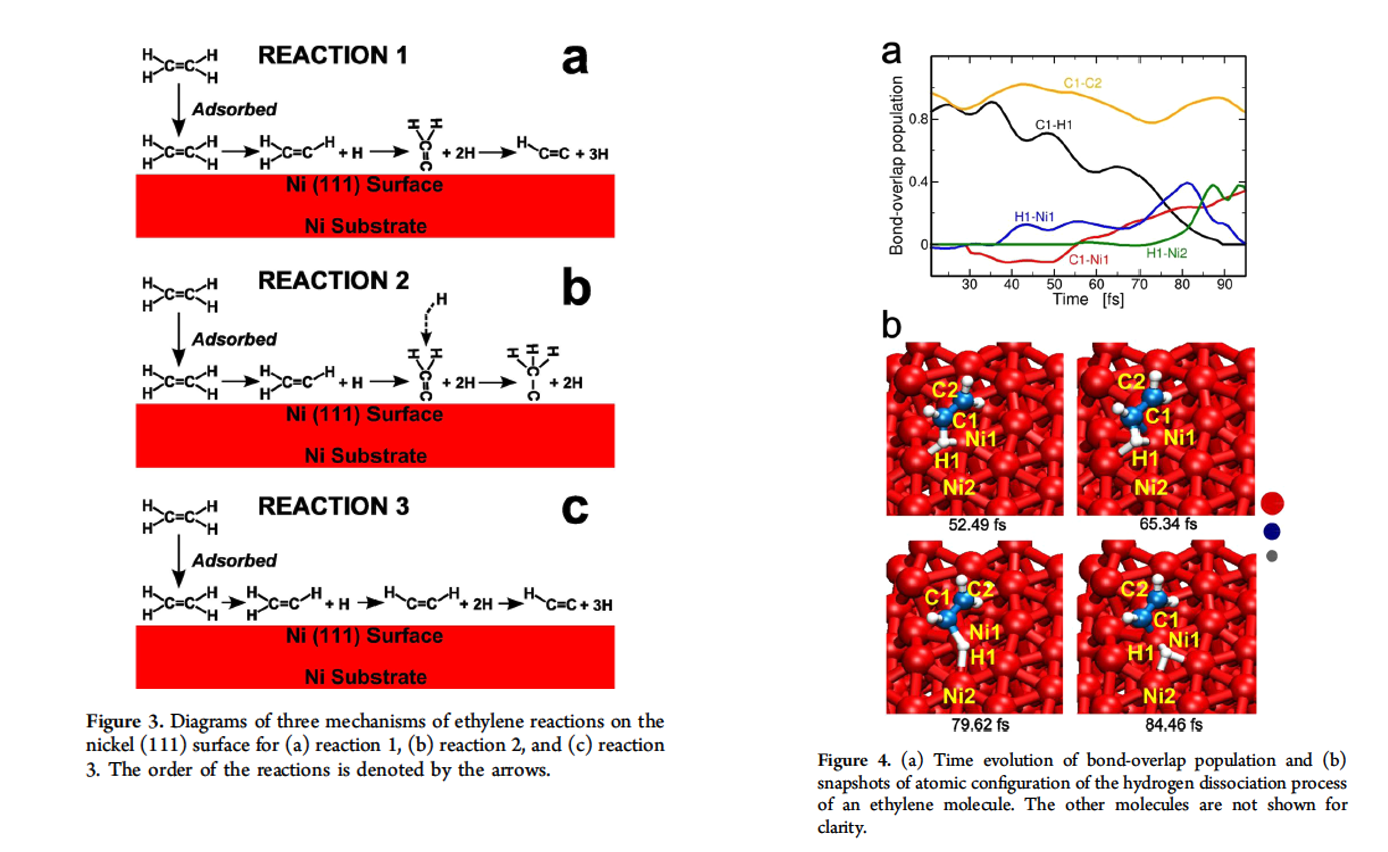
\includegraphics[width=0.6\linewidth]{lectures/figures/13-Surface_reactions.png}
            \caption{AIMD of ethylene reaction on Ni(111).\cite{arifinInitioMolecularDynamics2015}}
        \end{figure}
    \end{frame}


    \begin{frame}[allowframebreaks]{Bibliography}
        \bibliographystyle{unsrt}
        \bibliography{refs}
    \end{frame}



    \begin{frame}
        \Huge{\centerline{The End}}
    \end{frame}

\end{document}

